\begin{figure}[!tbp]
  \centering
  \subfloat[alpha 1]{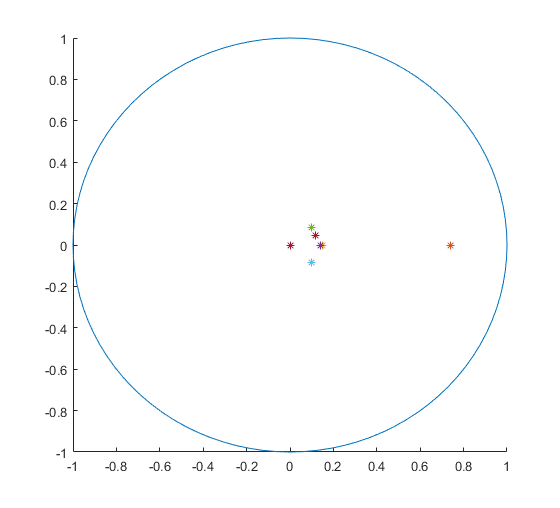
\includegraphics[width=0.5\textwidth]{Tekeningen/GMRES_alpha1_eigenv}\label{alpha 1}}
  \hfill
  \subfloat[alpha 5]{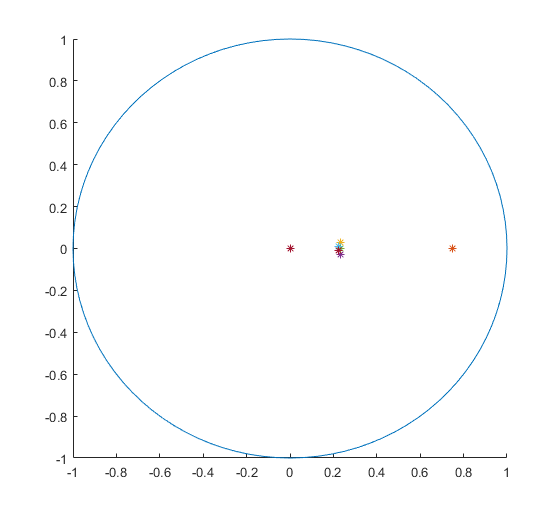
\includegraphics[width=0.5\textwidth]{Tekeningen/GMRES_alpha5_eigenv}\label{alpha 5}}
  \caption{Links eigenwaarden voor $\alpha = 1$, rechts voor $\alpha = 5$}
\end{figure}

\begin{figure}[!tbp]
  \centering
  \subfloat[alpha 10]{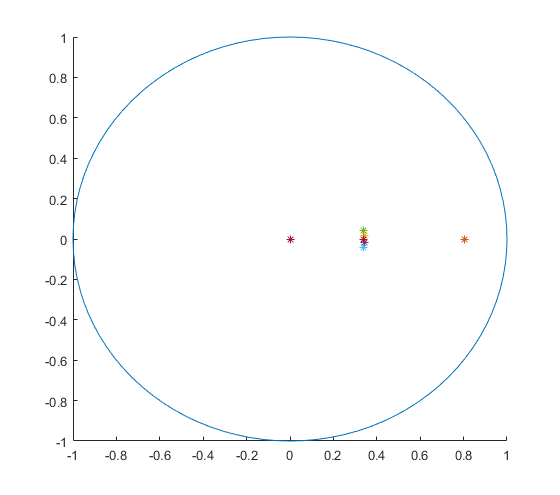
\includegraphics[width=0.5\textwidth]{Tekeningen/GMRES_alpha10_eigenv}\label{alpha 10}}
  \hfill
  \subfloat[alpha 100]{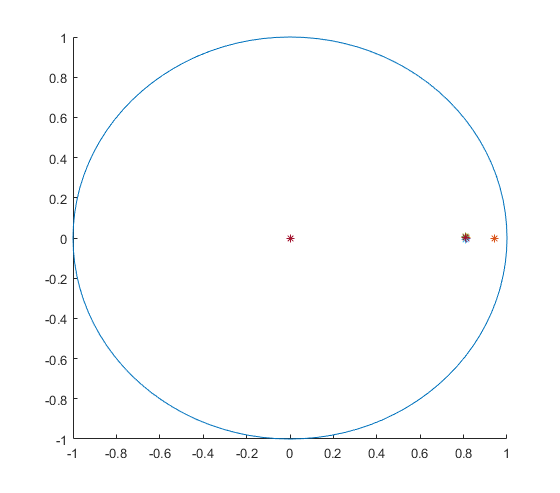
\includegraphics[width=0.5\textwidth]{Tekeningen/GMRES_alpha100_eigenv}\label{alpha 100}}
  \caption{Links eigenwaarden voor $\alpha = 10$, rechts voor $\alpha = 100$}
\end{figure}

\begin{figure}[!tbp]
  \centering
  \subfloat[fout op $\|r_{n}\|$]{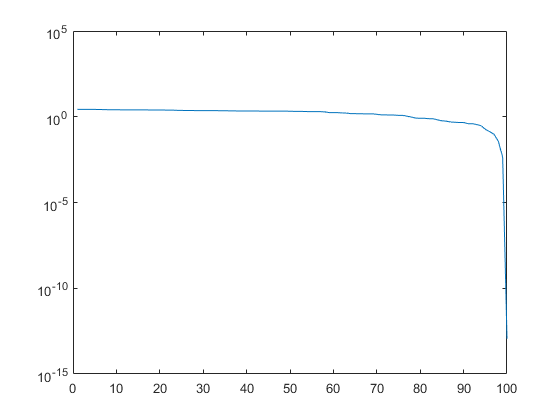
\includegraphics[width=0.5\textwidth]{Tekeningen/GMRES_alpha1_r}\label{r_1}}
  \hfill
  \subfloat[fout op exacte oplossing]{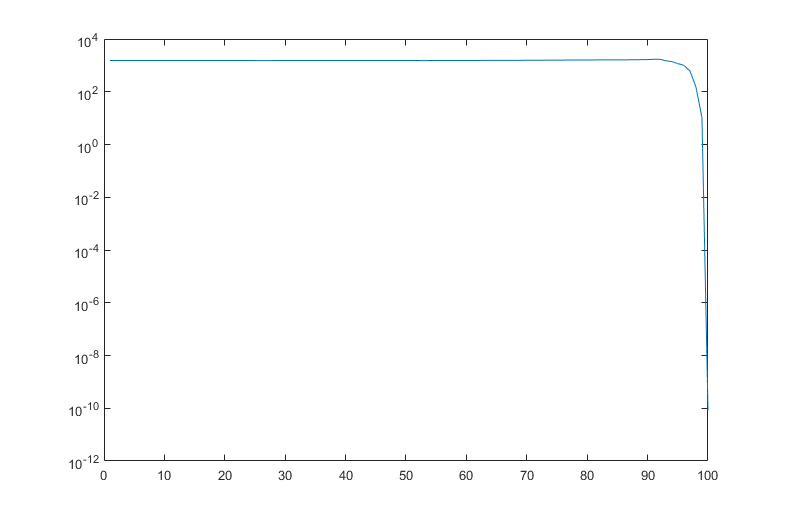
\includegraphics[width=0.5\textwidth]{Tekeningen/GMRES_alpha1_x-y}\label{x-y_1}}
  \caption{Resp. fouten voor $\alpha = 1$.}
\end{figure}

\begin{figure}[!tbp]
  \centering
  \subfloat[fout op $\|r_{n}\|$]{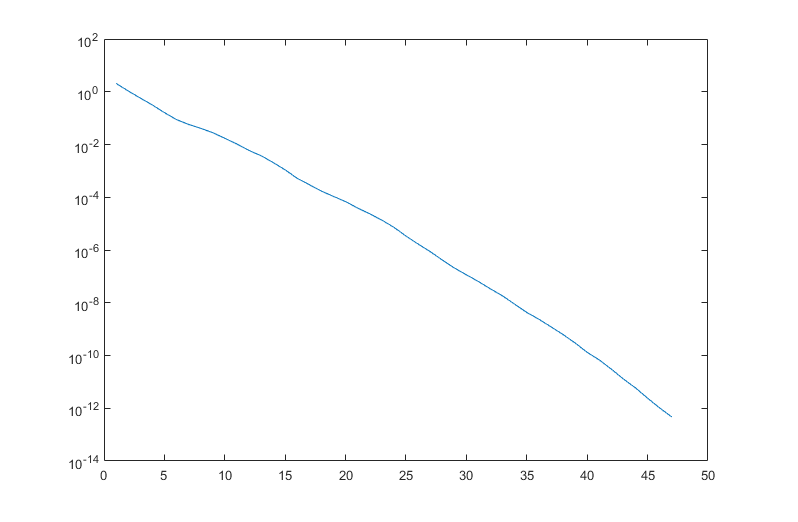
\includegraphics[width=0.5\textwidth]{Tekeningen/GMRES_alpha5_r}\label{r_5}}
  \hfill
  \subfloat[fout op exacte oplossing]{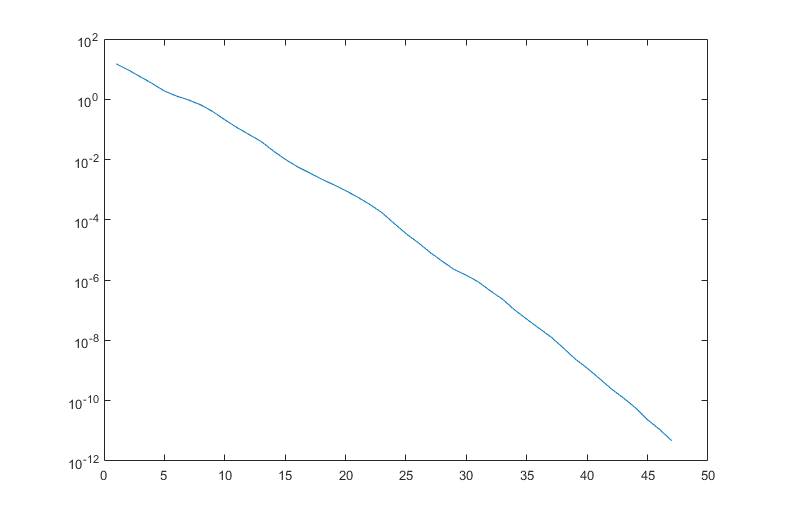
\includegraphics[width=0.5\textwidth]{Tekeningen/GMRES_alpha5_x-y}\label{x-y_5}}
  \caption{Resp. fouten voor $\alpha = 5$.}
\end{figure}

\begin{figure}[!tbp]
  \centering
  \subfloat[fout op $\|r_{n}\|$]{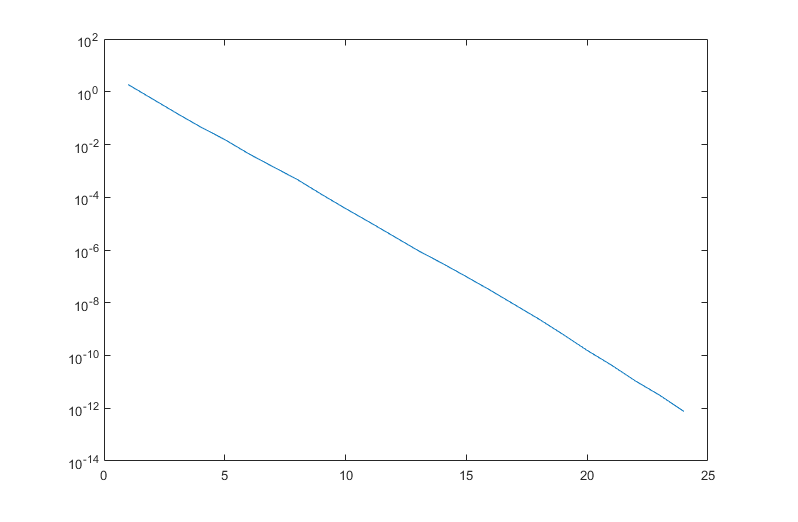
\includegraphics[width=0.5\textwidth]{Tekeningen/GMRES_alpha10_r}\label{r_10}}
  \hfill
  \subfloat[fout op exacte oplossing]{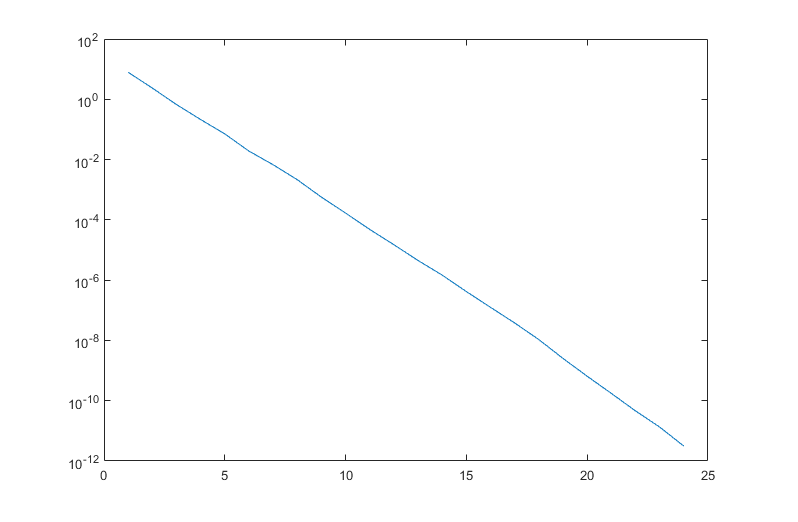
\includegraphics[width=0.5\textwidth]{Tekeningen/GMRES_alpha10_x-y}\label{x-y_10}}
  \caption{Resp. fouten voor $\alpha = 10$.}
\end{figure}

\begin{figure}[!tbp]
  \centering
  \subfloat[fout op $\|r_{n}\|$]{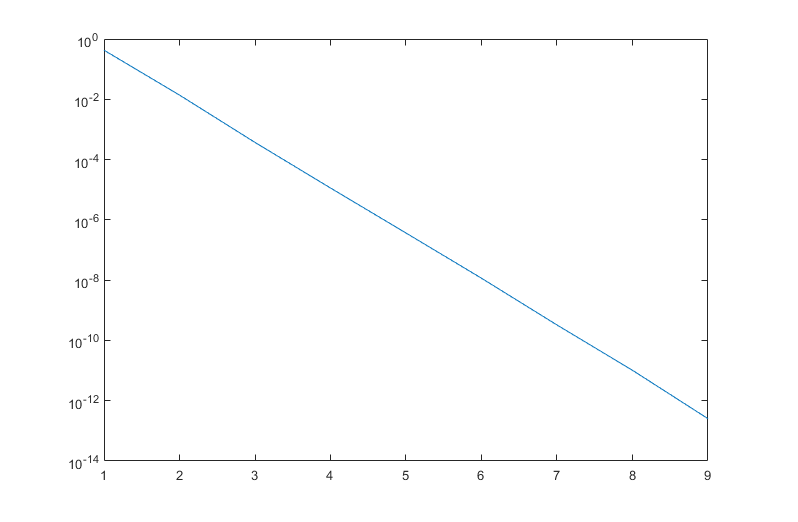
\includegraphics[width=0.5\textwidth]{Tekeningen/GMRES_alpha100_r}\label{r_100}}
  \hfill
  \subfloat[fout op exacte oplossing]{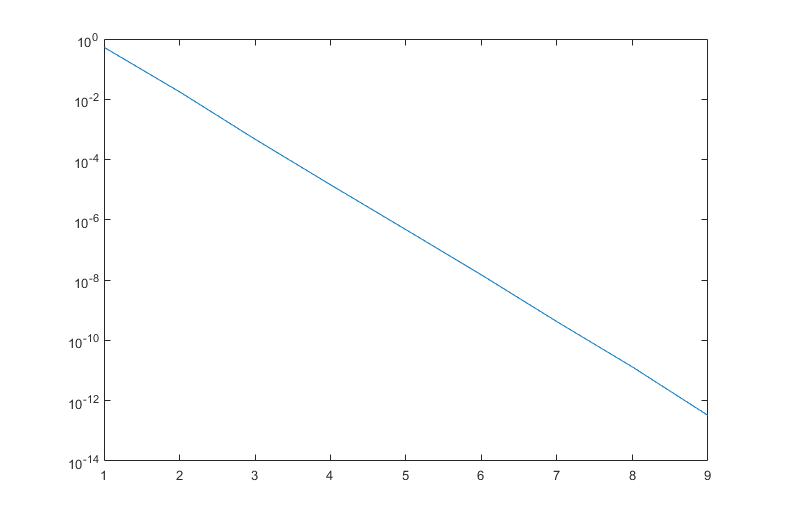
\includegraphics[width=0.5\textwidth]{Tekeningen/GMRES_alpha100_x-y}\label{x-y_100}}
  \caption{Resp. fouten voor $\alpha = 100$.}
\end{figure}


